\documentclass[11pt,a4paper]{article}

% Datos de la entrega
\newcommand{\codigoactividad}{TA-PFC-E1}
\newcommand{\nombreactividad}{Proyecto Fin de Curso, entrega 1: definición, requisitos y arquitectura base del sistema distribuido}
\newcommand{\nombreproyecto}{Sistema de gestión de documentos de pre-sustentaciones de trabajos de titulación}
\newcommand{\integrantes}{Benites Pérez Dariem Alberto \\ Castro Coello Mario Sebastián \\ Cedeño Intriago Jilmar Jesús \\ Pozo Castillo Steven Fernando}
\newcommand{\repositorio}{https://github.com/reyshadow0/isr701-pfc}
\newcommand{\fechaentrega}{22 de noviembre de 2026}

\usepackage[T1]{fontenc}
\usepackage[utf8]{inputenc}
\usepackage[spanish,es-tabla,es-nodecimaldot]{babel}
\usepackage{lmodern}
\usepackage{microtype}
\usepackage[a4paper,margin=2.5cm]{geometry}
\usepackage{graphicx}
\usepackage{booktabs}
\usepackage{tabularx}
\usepackage{longtable}
\usepackage{float}
\usepackage{xcolor}
\usepackage{listings}
\usepackage{csquotes}
\usepackage[backend=biber,style=ieee]{biblatex}
\addbibresource{referencias.bib}
\usepackage[hidelinks]{hyperref}

\graphicspath{{figuras/}{diagramas/}}

% Permite cortar URL largas en la bibliografía (evita desbordes)
\setcounter{biburlnumpenalty}{100}
\setcounter{biburlucpenalty}{100}
\setcounter{biburllcpenalty}{100}

\lstset{
  basicstyle=\ttfamily\small,
  breaklines=true,
  frame=single,
  numbers=left,
  numberstyle=\tiny,
  showstringspaces=false,
  extendedchars=true,
  literate={á}{{\'a}}1 {é}{{\'e}}1 {í}{{\'i}}1 {ó}{{\'o}}1 {ú}{{\'u}}1
           {Á}{{\'A}}1 {É}{{\'E}}1 {Í}{{\'I}}1 {Ó}{{\'O}}1 {Ú}{{\'U}}1
           {ñ}{{\~n}}1 {Ñ}{{\~N}}1 {ü}{{\"u}}1 {¿}{{?`}}1 {¡}{{!`}}1
}
\renewcommand{\lstlistingname}{Código}

\hypersetup{pdftitle={\codigoactividad: \nombreproyecto}}

\begin{document}

\begin{titlepage}
  \centering
  {\large\bfseries UNIVERSIDAD TÉCNICA ESTATAL DE QUEVEDO\par}
  \vspace{0.3cm}
  {Facultad de Ciencias de la Computación\par}
  {Carrera de Software\par}
  \vspace{2cm}
  {\large Aplicaciones Distribuidas (ISR-701)\par}
  \vspace{1.2cm}
  {\Large\bfseries \nombreproyecto\par}
  \vspace{0.6cm}
  {\large \codigoactividad: \nombreactividad\par}
  \vfill
  \begin{tabular}{@{}ll@{}}
    \toprule
    \textbf{Integrante} & \textbf{Rol} \\
    \midrule
    Benites Pérez Dariem Alberto   & \\
    Castro Coello Mario Sebastián  & \\
    Cedeño Intriago Jilmar Jesús   & \\
    Pozo Castillo Steven Fernando  & \\
    \bottomrule
  \end{tabular}
  \par\vspace{1cm}
  \begin{tabular}{@{}rl@{}}
    \textbf{Docente:}          & Gleiston Cicerón Guerrero Ulloa, PhD \\
    \textbf{Nivel / paralelo:} & Séptimo nivel / B \\
    \textbf{Periodo:}          & SPA 2026--2027 \\
    \textbf{Fecha de entrega:} & \fechaentrega \\
  \end{tabular}
  \par\vspace{1cm}
  {\small Repositorio: \url{\repositorio}\par}
\end{titlepage}

\tableofcontents
\newpage

\section{Resumen ejecutivo}

Este proyecto propone un sistema distribuido para gestionar los documentos y
las actividades de las pre-sustentaciones de trabajos de titulación de la
carrera de Software de la Universidad Técnica Estatal de Quevedo. Actualmente,
parte del proceso se coordina de manera manual y por correo electrónico. Las
actas se solicitan y entregan por ese medio, las firmas en papel retrasan el
cierre y cambios importantes, como la sustitución de un tutor, pueden quedar
sin registro. La entrevista realizada a la Ing. Nancy Rodríguez permitió
precisar que normalmente participan entre 10 y 12 estudiantes por periodo y
que la calificación, el acta y el porcentaje de similitud son datos críticos.

La propuesta cubre el registro y seguimiento de solicitudes, la entrega de
informes en PDF y reportes de URKUND, la asignación de tutores y tribunales, el
registro de evaluaciones, la consolidación de la nota y la generación del acta.
Se definieron doce historias de usuario y requisitos no funcionales orientados
a rendimiento, disponibilidad, seguridad, integridad y facilidad de uso. La
nota final combina el 40\% del tribunal con el 60\% del docente de Desarrollo
de Titulación II; por ello, las calificaciones y las actas requieren
consistencia, mientras que avisos, listados y reportes admiten una actualización
no inmediata.

La arquitectura se documentó mediante los niveles de contexto y contenedores
del modelo C4. Los usuarios acceden desde una aplicación web Angular a través
de un API Gateway. La solución separa cinco servicios Spring Boot: Usuarios,
Cronograma, Solicitudes y documentos, Evaluación y actas, y Notificaciones.
Cada servicio administra su propia base PostgreSQL; los documentos se almacenan
en MinIO y RabbitMQ distribuye los eventos que no necesitan respuesta
inmediata. Esta separación busca que una falla en notificaciones o cronograma
no impida registrar evaluaciones durante la semana de predefensas. Los ADR
justifican el estilo de microservicios y la combinación de comunicación
síncrona y asíncrona.

El análisis contempla riesgos de interrupción en la carga de documentos,
lecturas de notas desactualizadas, caída de componentes compartidos, cambios
defectuosos en reglas y saturación de la API. Las mitigaciones incluyen
validación de archivos, lectura de la fuente principal para generar actas,
despliegues graduales, versionado de reglas, acceso administrativo independiente
y límites de solicitudes. Como resultado de esta primera entrega quedan
establecidos el problema, los requisitos, la arquitectura base, las decisiones
técnicas, los riesgos y un esqueleto funcional de los servicios principales.

\section{Contexto y problema}

La carrera de Software de la Universidad Técnica Estatal de Quevedo realiza
pre-sustentaciones como parte de Desarrollo de Titulación II. En este proceso
participan el estudiante, el docente de la asignatura, el director del trabajo,
la coordinación de titulación y un tribunal formado por un presidente y dos
miembros. Durante el segundo periodo 2024--2025 se registraron 12 estudiantes;
dos se retiraron y diez llegaron a la predefensa. Por tanto, el volumen habitual
es de 10 a 12 estudiantes por periodo.

Actualmente, varias actividades se coordinan de forma manual y mediante correo
electrónico. Por ese medio se solicitan y entregan las actas, mientras que la
firma en papel retrasa el cierre del proceso y deja abierta la posibilidad de
extravíos. También se recordó un cambio repentino de tutor que produjo
conflictos porque no quedó registrado. El sistema propuesto debe conservar una
bitácora de esos cambios y mostrar el estado de cada solicitud a las personas
autorizadas.

Cada estudiante presenta dos o tres documentos PDF: el informe del trabajo, el
reporte de URKUND que incorpora el director y, cuando el tribunal formula
observaciones, una versión corregida. Con un máximo previsto de 20 MB por
archivo, el volumen de documentos entregados no supera los 720 MB para 12
estudiantes, sin contar las actas generadas. La carga se concentra en los días
anteriores a las predefensas y durante la semana 19 del décimo semestre.

La calificación y el acta son datos críticos. La nota final combina el 40\% del
tribunal y el 60\% del docente de Desarrollo de Titulación II, y luego se
registra en el sistema informático de la UTEQ. El porcentaje de URKUND también
afecta el resultado: por debajo del 10\% el trabajo se considera aceptable,
mientras que un valor superior al 20\% interrumpe la predefensa. Un error o una
versión desactualizada de estos datos puede cambiar la condición de aprobación
del estudiante.

Los principales interesados esperan resultados distintos: el estudiante
necesita entregar documentos y consultar el estado; coordinación requiere
organizar solicitudes, tutores, tribunales y reportes; el director debe adjuntar
el reporte de similitud; y el tribunal necesita revisar el expediente, registrar
su evaluación y completar el acta. Los avisos por correo, los listados, los
reportes y el estado visible pueden aceptar una actualización no inmediata,
pero las notas y las actas deben mantenerse íntegras y actualizadas.

La información de esta sección procede del resumen reconstruido por el equipo
después de la entrevista del 19 de noviembre de 2026. La Ing. Nancy Rodríguez
confirmó el contenido del resumen utilizado como fuente.

\section{Objetivos}

\subsection{Objetivo general}

Desarrollar un sistema distribuido para gestionar los documentos de las
pre-sustentaciones de trabajos de titulación en la Universidad Técnica Estatal
de Quevedo, desde la entrega de la solicitud hasta la generación del acta
de predefensa y la consolidación de la nota final.

\textbf{Indicador.} Porcentaje de casos de prueba de extremo a extremo que
completan el flujo previsto, desde la entrega de documentos hasta la generación
del acta de predefensa y la consolidación de la nota final. \textbf{Meta.} Al menos el 85\%.

\subsection{Objetivos específicos}

\begin{enumerate}
    \item Implementar la entrega del informe de predefensa, el reporte de
    coincidencias de URKUND y el informe corregido cuando haya observaciones.
    La entrega del anteproyecto corresponde a una etapa previa.

    \textbf{Indicador.} Porcentaje de casos de prueba en los que el sistema
    acepta solicitudes con documentos válidos y detecta los documentos
    obligatorios faltantes. \textbf{Meta.} Al menos el 90\%.

    \item Facilitar la revisión de los documentos por parte de coordinación y
    permitir que el estudiante consulte el estado y las observaciones de su
    solicitud.

    \textbf{Indicador.} Porcentaje de solicitudes de prueba en las que el
    estado y las observaciones consultadas por el estudiante coinciden con lo
    registrado por coordinación. \textbf{Meta.} Al menos el 90\%.

    \item Registrar la calificación del tribunal según su rúbrica y
    consolidar la nota final con el 40\% del tribunal y el 60\% del docente
    de Desarrollo de Titulación II.
    En el proceso actual, el docente registra la nota final en el SGA.

    \textbf{Indicador.} Porcentaje de casos de prueba en los que la
    calificación del tribunal queda vinculada a la solicitud correcta y
    la nota final coincide con el cálculo esperado. \textbf{Meta.} Al menos el 95\%.

    \item Generar el acta de predefensa con las observaciones, la calificación
    vigente del tribunal y los espacios de firma del presidente y los dos
    miembros. Bloquear la generación si la calificación vigente no se
    puede verificar.

    \textbf{Indicador.} Porcentaje de casos de prueba que generan el acta
    correcta cuando la nota es verificable o bloquean la generación cuando
    no se puede verificar. \textbf{Meta.} Al menos el 95\%.
\end{enumerate}

\section{Trabajos relacionados}

Caldarelli y Ellul revisaron propuestas que utilizan blockchain para conservar
y verificar expedientes académicos. El estudio destaca la trazabilidad de los
registros, la reducción de intermediarios y la necesidad de identificar a la
institución que introduce la información en la cadena
\cite{Caldarelli2021}. El proyecto toma como referencia la importancia de una
bitácora auditable y de la integridad documental, pero no adopta blockchain:
conserva los documentos y eventos dentro de la infraestructura institucional y
se concentra en el flujo de pre-sustentaciones de la UTEQ.

Fekete y Kiss propusieron un sistema de educación superior basado en contratos
inteligentes y una arquitectura modular con zkEVM. Su propuesta busca que los
documentos y las interacciones académicas puedan verificarse a lo largo del
tiempo, con énfasis en seguridad, descentralización e interoperabilidad
\cite{Fekete2023}. De este trabajo se toma la separación de responsabilidades y
la necesidad de registrar cada interacción relevante. La diferencia es que el
sistema de este proyecto emplea servicios web y autenticación institucional,
sin billeteras ni transacciones en una red blockchain.

Satybaldy, Subedi y Nowostawski diseñaron un marco para verificar documentos en
línea mediante identidad autosoberana y credenciales verificables. Su prueba de
concepto prioriza privacidad, interoperabilidad y verificación sin depender de
un intermediario \cite{Satybaldy2022}. El proyecto toma como referencia la
protección de los documentos y el control de acceso por actor, pero su alcance
es diferente: administra solicitudes, informes, evaluaciones y actas dentro de
un procedimiento universitario concreto, en vez de crear credenciales
portables para múltiples organizaciones.

Los tres trabajos muestran mecanismos para preservar confianza y trazabilidad
en documentos digitales. Ninguno integra, dentro del proceso específico de una
pre-sustentación de la UTEQ, la entrega del informe y del reporte de similitud,
el seguimiento de la solicitud, la evaluación del tribunal y la generación del
acta. Ese flujo institucional constituye la diferencia principal del sistema
propuesto.

\section{Requisitos}

\subsection{Requisitos no funcionales}

Las características de calidad corresponden a ISO/IEC 25010:2023.

\begin{description}
    \item[RNF-01. Capacidad documental.] Dimensionar el sistema para 10 a
    12 estudiantes por periodo y hasta tres PDF por estudiante, con un límite
    de 20 MB por archivo. El máximo previsto de archivos cargados es de
    720 MB por periodo (12 estudiantes por 3 archivos por 20 MB), a lo que
    se suma el espacio de las actas generadas. La nómina del segundo periodo
    2024--2025 tuvo 12 estudiantes inscritos y 10 presentaron. Verificar la
    capacidad con ese volumen y probar el límite de tamaño por archivo.
    \textbf{Característica.} Eficiencia de desempeño (capacidad).

    \item[RNF-02. Disponibilidad.] Alcanzar una disponibilidad mensual de al
    menos 99,5\% fuera de la semana de predefensas. Durante esa semana,
    recuperar las funciones críticas en un máximo de 60 minutos consecutivos
    por interrupción. Verificar ambos criterios con registros de monitoreo.
    Si el sistema no está disponible, el tribunal puede continuar la
    predefensa y registrar las calificaciones después.
    \textbf{Característica.} Fiabilidad (disponibilidad y recuperabilidad).

    \item[RNF-03. Acceso desde computadora y celular.] Permitir la carga de
    documentos, la revisión de informes y la consulta del estado desde
    ambos tipos de dispositivo, según el rol. Verificar esas operaciones
    en 2 entornos: un navegador de escritorio y uno móvil.
    \textbf{Característica.} Flexibilidad (adaptabilidad).

    \item[RNF-04. Conservación documental.] Conservar permanentemente las
    actas y las notas del expediente académico. Aplicar a los demás
    documentos el plazo de la tabla institucional de conservación
    documental, pendiente de confirmar. El proceso automático de limpieza
    debe eliminar 0 actas y 0 registros de notas. Verificarlo ejecutando
    ese proceso sobre expedientes de prueba.
    \textbf{Característica.} Seguridad (integridad).

    \item[RNF-05. Concurrencia.] Soportar 30 usuarios simultáneos en una
    prueba de carga que combine entrega de archivos, revisión de informes y
    consulta del estado, con 0 errores atribuibles a saturación durante la
    prueba. Los 30 usuarios son una meta preliminar de diseño basada en la
    estimación de pocas decenas de usuarios durante las predefensas, que se realizan en la semana 19 del décimo semestre, y en los días previos de entrega.
    \textbf{Característica.} Eficiencia de desempeño (capacidad).

    \item[RNF-06. Confidencialidad.] Permitir 0 accesos no autorizados a
    informes y calificaciones. Verificar, con al menos 2 expedientes y
    2 tribunales de prueba, que un estudiante no pueda acceder a un
    expediente ajeno y que un tribunal no pueda acceder a expedientes
    asignados al otro tribunal.
    \textbf{Característica.} Seguridad (confidencialidad).
\end{description}

\section{Justificación de la arquitectura distribuida}
\label{sec:justificacion}

\section{Arquitectura base (modelo C4)}

Describimos el sistema con los dos primeros niveles del modelo C4: el diagrama de contexto (nivel~1) y el de contenedores (nivel~2). Los dos se hicieron en draw.io, y los archivos editables y sus exportaciones están en \nolinkurl{docs/diagramas/}. En los diagramas y en este documento el sistema se llama \emph{Sistema de gestión de pre-sustentaciones}.

\subsection{Del primer bosquejo al diagrama C4}

La arquitectura empezó como un bosquejo a mano del 20 de noviembre de 2026 (figura~\ref{fig:bosquejo}). Ese bosquejo ya tenía los cinco actores, la aplicación web, el API Gateway, los cinco servicios, cuatro bases de datos, el almacenamiento de los PDF y la cola de mensajes. Al pasarlo a C4 hicimos cinco cambios:

\begin{itemize}
  \item agregamos la tecnología de cada contenedor y el protocolo de cada flecha;
  \item agregamos los sistemas externos del nivel~1: URKUND, el servicio de correo y el SGA;
  \item agregamos una llamada directa de Evaluación y actas a Solicitudes y documentos, porque antes de abrir la rúbrica hace falta saber si el informe y el reporte de URKUND ya están;
  \item le dimos a Notificaciones su propia base, para guardar los avisos enviados y los que faltan por enviar;
  \item guardamos el porcentaje de URKUND como un dato de la base de Solicitudes, y no solo dentro del PDF.
\end{itemize}

\begin{figure}[htbp]
  \centering
  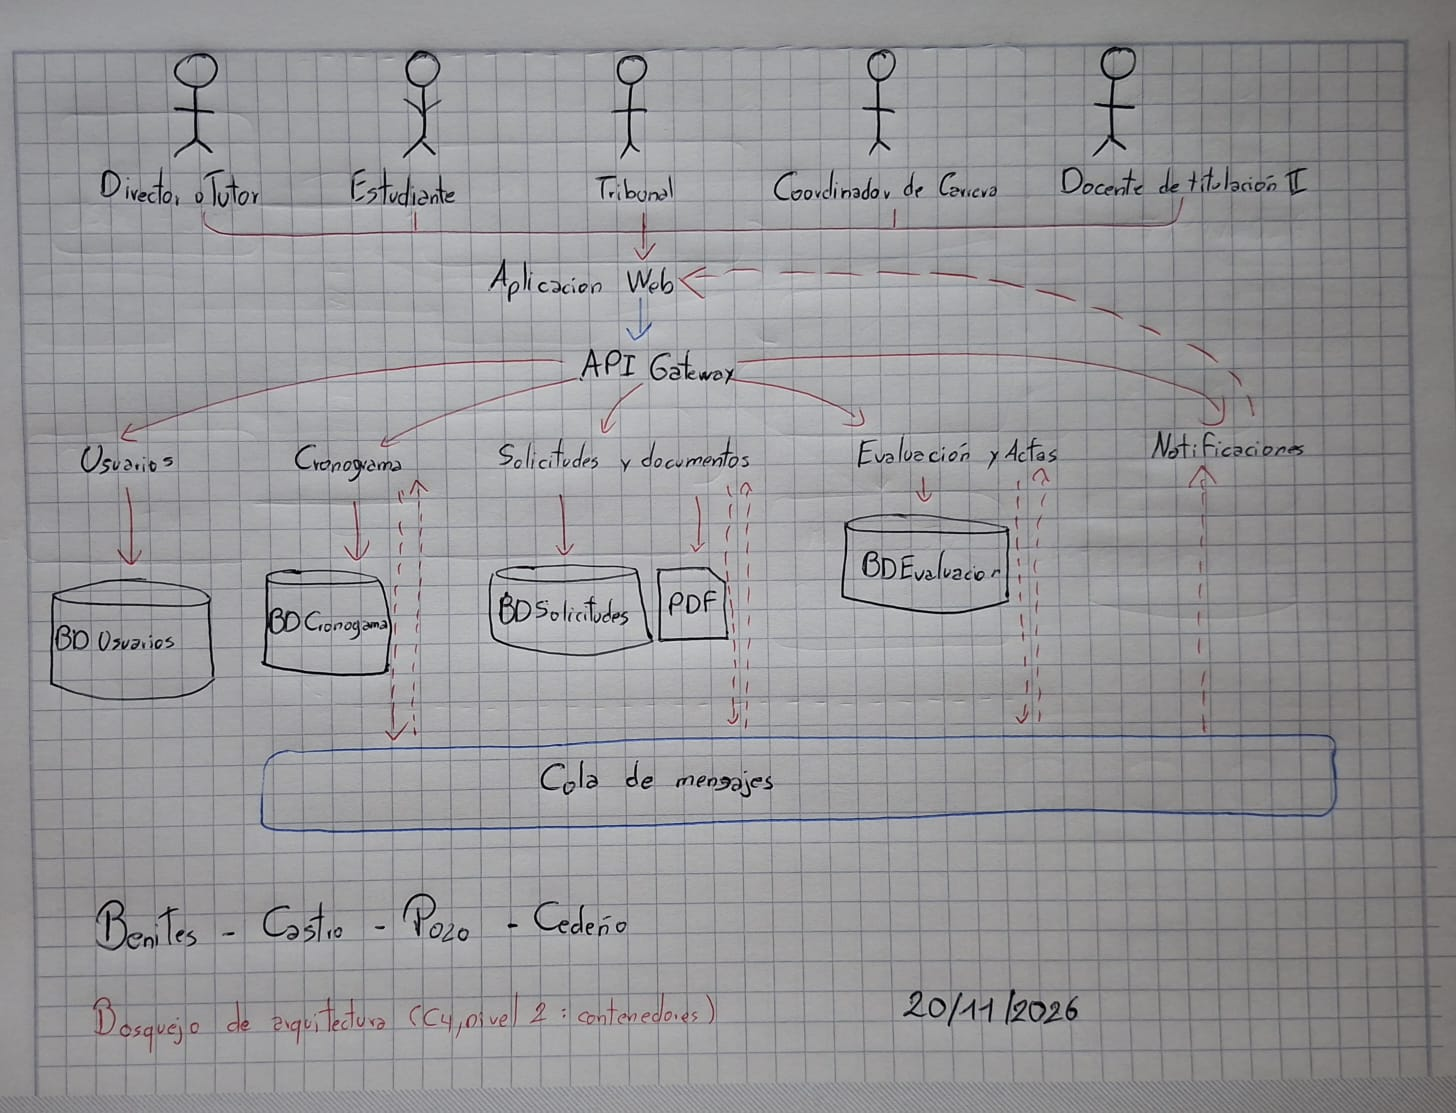
\includegraphics[width=0.68\textwidth]{../evidencias/fotos/primer-bosquejo-arquitectura-2026-11-20.jpeg}
  \caption{Primer bosquejo de la arquitectura, hecho a mano el 20 de noviembre de 2026.}
  \label{fig:bosquejo}
\end{figure}

\subsection{Nivel 1: contexto}

La figura~\ref{fig:c4-n1} muestra el sistema como una caja cerrada, con quienes lo usan y con los sistemas que están alrededor. Los cinco actores salen de la entrevista:

\begin{itemize}
  \item el estudiante sube su informe y el reporte de URKUND, y sigue su trámite;
  \item el director o tutor revisa el porcentaje de coincidencia en URKUND, lo registra en el sistema y sube sus informes;
  \item el tribunal, formado por un presidente y dos miembros, califica la predefensa con la rúbrica;
  \item el coordinador de carrera arma el cronograma;
  \item el docente de Titulación~II pone su 60~\% de la nota y consolida la nota final.
\end{itemize}

El sistema solo se comunica con el servicio de correo, por SMTP, para enviar los avisos. Con URKUND y con el SGA no se conecta: el director usa URKUND por fuera, y el docente de Titulación~II registra la nota final en el SGA a mano, como se hace hoy. La aprobación del anteproyecto queda fuera del alcance porque es una etapa previa. La secretaría tampoco aparece, porque se encarga del acta de la sustentación final y no de la predefensa.

\begin{figure}[htbp]
  \centering
  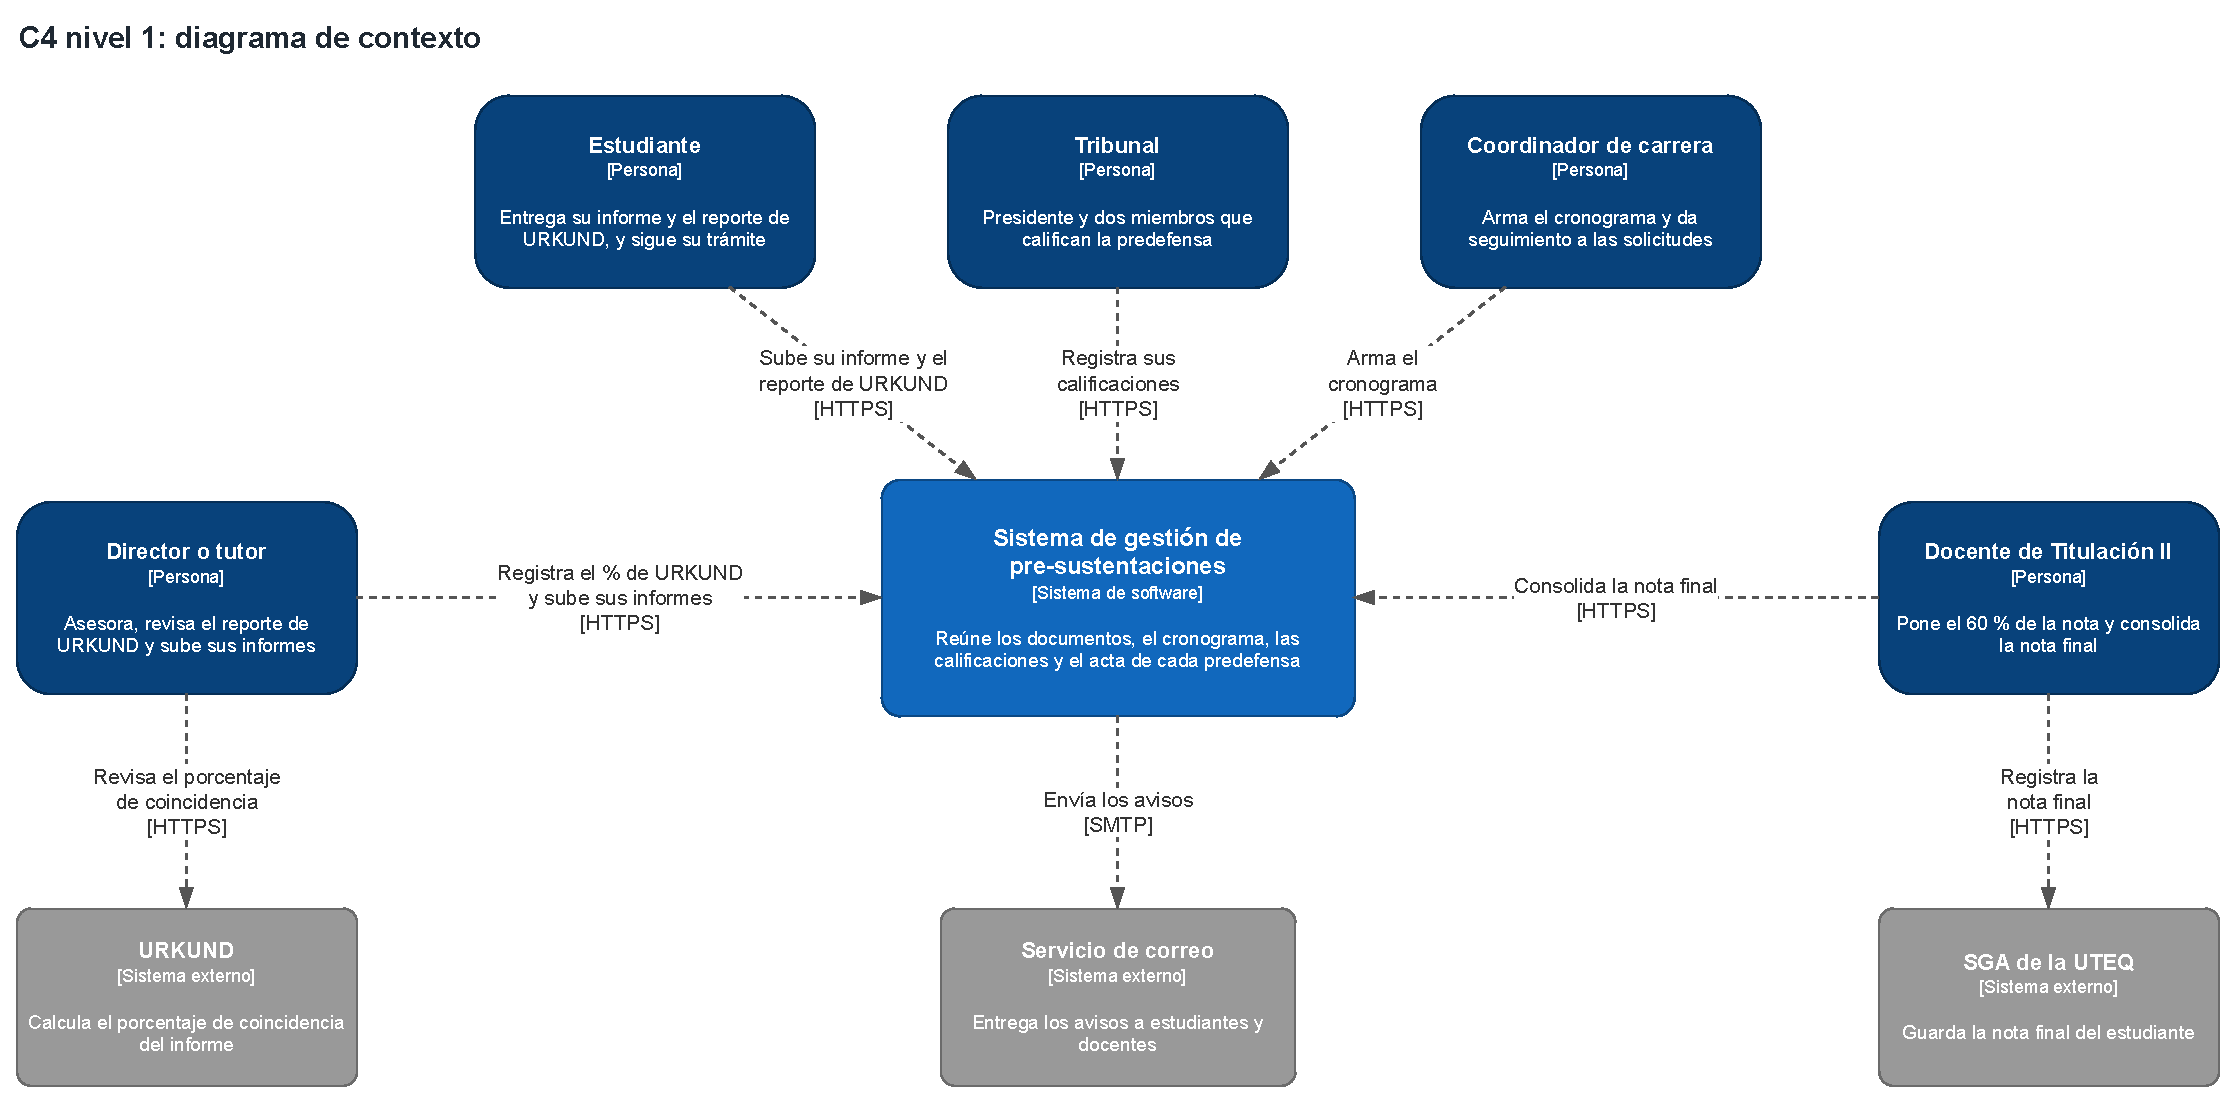
\includegraphics[width=\textwidth]{c4-nivel1-contexto.pdf}
  \caption{C4 nivel 1: diagrama de contexto.}
  \label{fig:c4-n1}
\end{figure}

\subsection{Nivel 2: contenedores}

La figura~\ref{fig:c4-n2} abre la caja del sistema. Los usuarios entran desde el navegador a la aplicación web, que manda cada petición al API Gateway con el JWT de la sesión. El gateway valida el JWT y envía la petición al servicio que corresponde. La tabla~\ref{tab:contenedores} resume cada contenedor.

\begin{figure}[htbp]
  \centering
  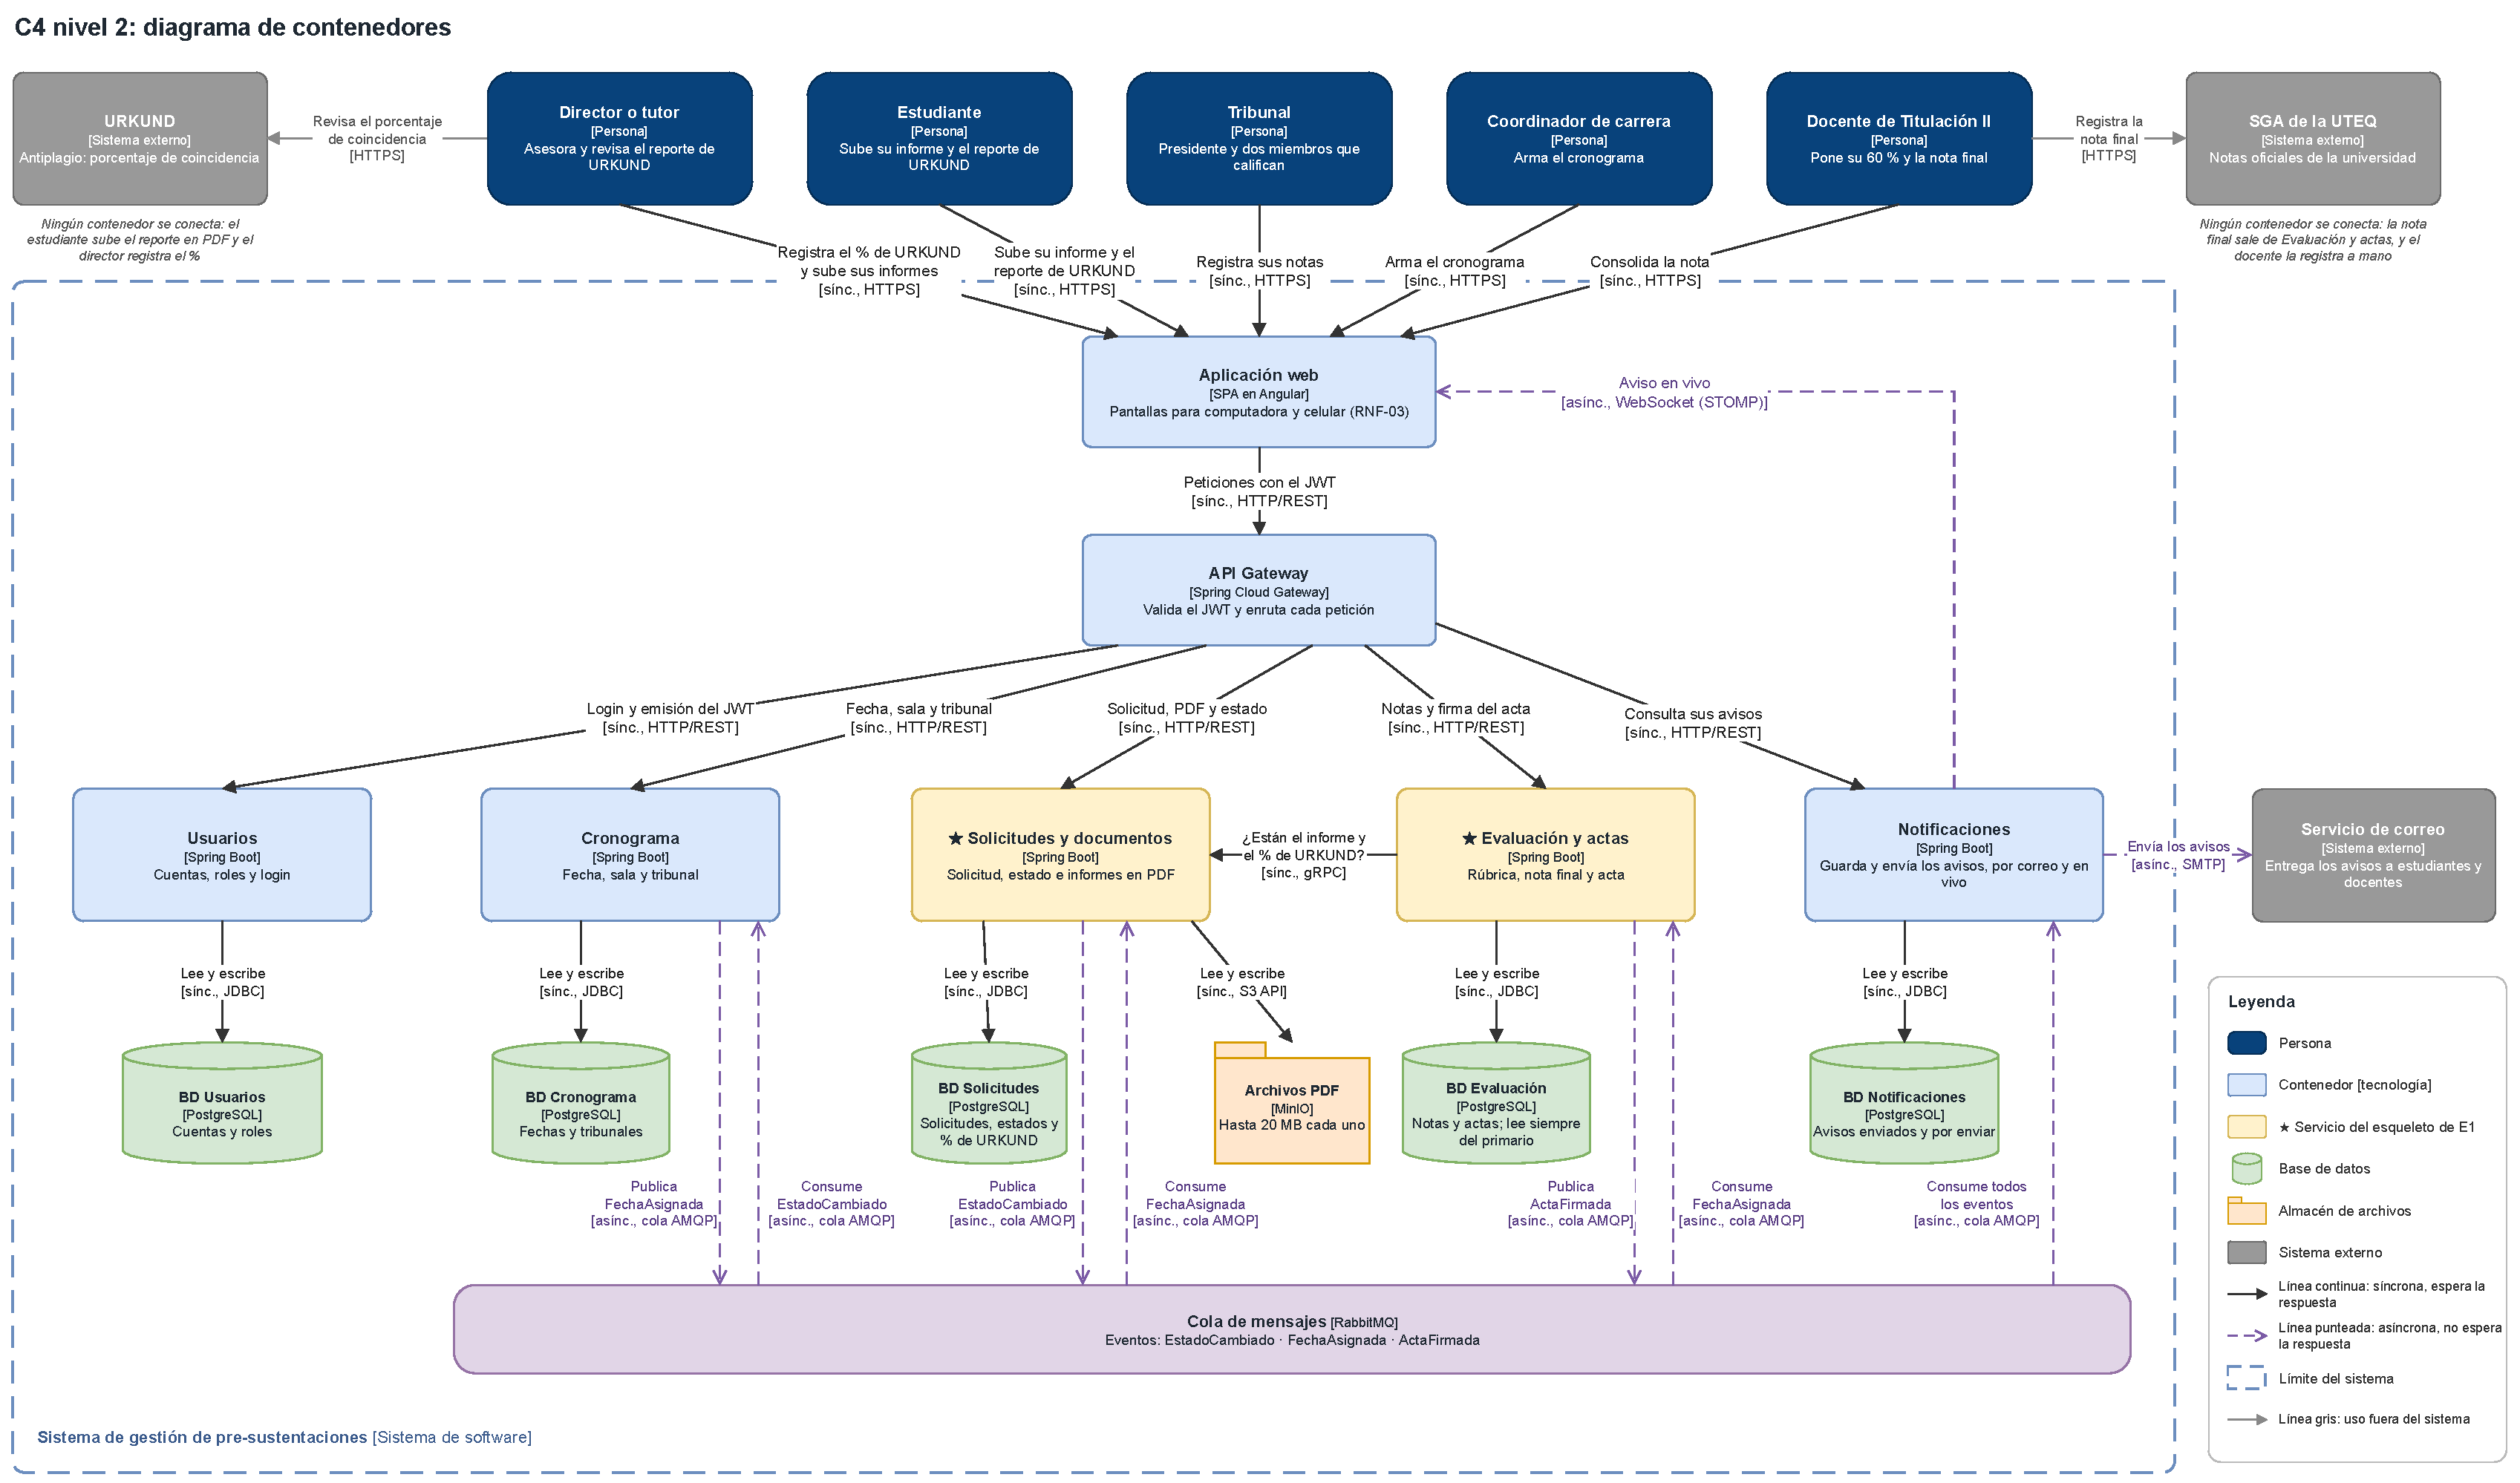
\includegraphics[width=\textwidth]{c4-nivel2-contenedores.pdf}
  \caption{C4 nivel 2: diagrama de contenedores. Las líneas continuas son llamadas síncronas y las punteadas, asíncronas.}
  \label{fig:c4-n2}
\end{figure}

\begin{table}[htbp]
  \centering
  \caption{Contenedores del sistema.}
  \label{tab:contenedores}
  \small
  \begin{tabularx}{\textwidth}{@{}>{\raggedright\arraybackslash}p{2.9cm} >{\raggedright\arraybackslash}p{2.6cm} >{\raggedright\arraybackslash}X >{\raggedright\arraybackslash}p{2.6cm}@{}}
    \toprule
    \textbf{Contenedor} & \textbf{Tecnología} & \textbf{Qué hace} & \textbf{Datos} \\
    \midrule
    Aplicación web & Angular & Pantallas para computadora y celular (RNF-03) & --- \\
    API Gateway & Spring Cloud Gateway & Única entrada: valida el JWT y enruta cada petición & --- \\
    Usuarios & Spring Boot & Cuentas, roles, inicio de sesión y emisión del JWT & BD Usuarios \\
    Cronograma & Spring Boot & Fecha, sala y tribunal de cada predefensa & BD Cronograma \\
    Solicitudes y documentos & Spring Boot & Solicitud, estado, informes en PDF y porcentaje de URKUND & BD Solicitudes y MinIO \\
    Evaluación y actas & Spring Boot & Rúbrica, nota final (40~\% del tribunal y 60~\% del docente) y acta & BD Evaluación \\
    Notificaciones & Spring Boot & Avisos por correo y en vivo & BD Notificaciones \\
    Cola de mensajes & RabbitMQ & Eventos \texttt{EstadoCambiado}, \texttt{FechaAsignada} y \texttt{ActaFirmada} & --- \\
    \bottomrule
  \end{tabularx}
\end{table}

Las bases de datos usan PostgreSQL. Cada servicio tiene la suya, y ningún servicio lee la base de otro: si necesita un dato, se lo pide al servicio dueño o lo recibe por un evento. Los PDF van en MinIO, fuera de las bases. Solicitudes y documentos y Evaluación y actas, marcados con una estrella en la figura, son los dos servicios del esqueleto de esta entrega (sección~13). El tipo y el mecanismo de cada interacción están en la sección~8, y lo que se prioriza con cada dato crítico, en la sección~9.

\section{Modelo de comunicación entre servicios}
\label{sec:comunicacion}

La regla es la misma del ADR-002: REST de la aplicación web al API Gateway y del gateway a cada servicio, gRPC cuando un servicio le pregunta algo a otro, y eventos por una cola de mensajes con AMQP (RabbitMQ). Para elegir entre síncrono y asíncrono usamos un criterio simple:

\begin{itemize}
  \item \textbf{síncrona}, cuando la respuesta decide el siguiente paso o hay una persona esperando en la pantalla;
  \item \textbf{asíncrona}, cuando el que envía no necesita esperar y un retraso es aceptable, como dijo la entrevistada para los avisos, el estado visible y los reportes.
\end{itemize}

La tabla~\ref{tab:comunicacion} recorre cada interacción del diagrama de contenedores (figura~\ref{fig:c4-n2}).

\begingroup
\footnotesize
\begin{xltabular}{\textwidth}{@{}>{\raggedright\arraybackslash}p{3.4cm} >{\raggedright\arraybackslash}p{1.5cm} >{\raggedright\arraybackslash}p{2.2cm} >{\raggedright\arraybackslash}X@{}}
    \caption{Tipo y mecanismo de cada interacción.}
    \label{tab:comunicacion} \\
    \toprule
    \textbf{Interacción} & \textbf{Tipo} & \textbf{Mecanismo} & \textbf{Por qué} \\
    \midrule
    \endfirsthead
    \multicolumn{4}{@{}l}{\emph{Tabla~\ref{tab:comunicacion} (continuación)}} \\
    \toprule
    \textbf{Interacción} & \textbf{Tipo} & \textbf{Mecanismo} & \textbf{Por qué} \\
    \midrule
    \endhead
    \bottomrule
    \endlastfoot
    Aplicación web $\rightarrow$API Gateway & Síncrona & HTTP/REST con JSON, sobre HTTPS & Es lo que habla el navegador, y la persona espera la respuesta en la pantalla. Cada petición lleva el JWT. \\
    \addlinespace
    API Gateway $\rightarrow$Usuarios, Cronograma, Solicitudes, Evaluación y Notificaciones & Síncrona & HTTP/REST & El gateway valida el JWT y reenvía la misma petición al servicio que corresponde, sin cambiar el formato. \\
    \addlinespace
    Evaluación y actas $\rightarrow$Solicitudes y documentos & Síncrona & gRPC & Antes de abrir la rúbrica, Evaluación pregunta si el informe y el reporte de URKUND están, y cuál es el porcentaje. La respuesta decide si se puede calificar, y ese dato tiene que ser exacto (sección~\ref{sec:cap-pacelc}). El contrato queda fijo en un archivo \texttt{.proto} que comparten los dos servicios. \\
    \addlinespace
    Cada servicio $\rightarrow$su base PostgreSQL & Síncrona & JDBC & El servicio necesita el dato para responder. Cada base es solo de su servicio. \\
    \addlinespace
    Solicitudes y documentos $\rightarrow$MinIO & Síncrona & API de S3 sobre HTTP & La entrega se confirma solo cuando el PDF quedó guardado (riesgo R01). \\
    \addlinespace
    Cronograma publica \texttt{FechaAsignada}; la consumen Solicitudes, Evaluación y Notificaciones & Asíncrona & Cola de mensajes, AMQP & Cronograma no tiene que esperar a los demás. Cada uno guarda la fecha, la sala y el tribunal que necesita, y si alguno está caído, el evento lo espera en la cola. \\
    \addlinespace
    Solicitudes publica \texttt{EstadoCambiado}; la consumen Cronograma y Notificaciones & Asíncrona & Cola de mensajes, AMQP & El cambio de estado no se detiene si otro servicio falla. El estado visible puede tardar unos segundos, y eso es aceptable. \\
    \addlinespace
    Evaluación publica \texttt{ActaFirmada}; la consume Notificaciones & Asíncrona & Cola de mensajes, AMQP & Firmar el acta no depende de que el aviso salga en ese momento. \\
    \addlinespace
    Notificaciones $\rightarrow$aplicación web & Asíncrona & WebSocket con STOMP & El servidor empuja el aviso y la pantalla no tiene que preguntar a cada rato. \\
    \addlinespace
    Notificaciones $\rightarrow$servicio de correo & Asíncrona & SMTP & El correo es el canal que ya usan. Si el envío falla, el aviso queda en la base de Notificaciones y se vuelve a intentar. \\
\end{xltabular}
\endgroup

Así, una falla se queda donde ocurre. Si se cae Notificaciones o el servicio de correo, los eventos esperan en la cola y nadie más se detiene. Si se cae Solicitudes y documentos, no se suben PDF, y Evaluación no abre la rúbrica porque no puede confirmar el informe ni el porcentaje de URKUND. En ese caso, el tribunal califica en papel y registra la nota después, como se hace hoy. La única llamada directa entre servicios es la de Evaluación a Solicitudes, y es la que prueba el esqueleto de esta entrega.

\section{Análisis CAP y PACELC}

El teorema CAP dice que, cuando la red se parte (P), un sistema que guarda un dato en más de un lugar tiene que elegir entre consistencia (C), es decir, que todos lean el último valor, y disponibilidad (A), es decir, que siempre responda~\cite{vanSteen2023}. PACELC agrega el caso normal: aun sin partición (E, de \emph{else}), hay que elegir entre baja latencia (L) y consistencia (C)~\cite{Abadi2012}. En nuestro sistema un dato está en más de un lugar en dos casos: cuando un servicio guarda una copia de un dato de otro, que le llega por eventos, y desde E3, cuando las bases tengan réplicas.

Para decidir usamos lo que dijo la entrevistada: es peor mostrar una nota desactualizada que no dejar registrarla por un rato, porque una nota vieja puede terminar en un acta firmada y en el SGA. La tabla~\ref{tab:pacelc} muestra la decisión para cada dato crítico.

\begin{table}[htbp]
  \centering
  \caption{Qué se prioriza con cada dato crítico.}
  \label{tab:pacelc}
  \footnotesize
  \begin{tabularx}{\textwidth}{@{}>{\raggedright\arraybackslash}p{2.4cm} >{\raggedright\arraybackslash}p{2.2cm} >{\raggedright\arraybackslash}p{1.5cm} >{\raggedright\arraybackslash}X >{\raggedright\arraybackslash}p{3.6cm}@{}}
    \toprule
    \textbf{Dato} & \textbf{Dueño} & \textbf{PACELC} & \textbf{Qué se prioriza} & \textbf{Qué le pasa al usuario} \\
    \midrule
    Notas por criterio y nota final & Evaluación y actas & PC/EC & Con partición, no se registra ni se muestra una nota que no se pueda confirmar en la base primaria. Sin partición, se lee siempre de la primaria, aunque tarde un poco más. & El tribunal puede tener que esperar, o anotar en papel y registrar después, como hoy. Nadie ve una nota vieja. \\
    \addlinespace
    Acta y sus firmas & Evaluación y actas & PC/EC & El acta se genera solo con las notas confirmadas en la base primaria (riesgo R02). & Si hay una falla, el acta se firma más tarde, pero nunca sale con una nota que falte. \\
    \addlinespace
    Porcentaje de URKUND & Solicitudes y documentos & PC/EC & Evaluación se lo pide por gRPC al dueño antes de abrir la rúbrica, en vez de usar una copia. Si Solicitudes no responde, la rúbrica no se abre. & El tribunal espera o califica en papel, pero nunca con un porcentaje equivocado. \\
    \addlinespace
    Fecha, sala y tribunal & Cronograma & PC/EC & Solo Cronograma asigna, y su base no deja guardar dos predefensas en la misma sala y hora, ni un docente en dos tribunales a la vez. Con partición no se asigna. & El coordinador no puede programar mientras dure la falla, pero no hay choques de horario. \\
    \addlinespace
    Informe en PDF & Solicitudes y documentos & PC/EC & La entrega se confirma solo cuando el archivo quedó guardado en MinIO (riesgo R01). & Si MinIO no responde, la solicitud queda en borrador y el estudiante vuelve a intentar. \\
    \addlinespace
    Estado visible, listados y reportes & Solicitudes y Cronograma, con copias en otros servicios & PA/EL & Se muestra el último dato recibido por eventos, aunque tenga unos segundos de atraso. & El estudiante o el coordinador pueden ver un estado o un reporte un poco atrasado. La entrevistada dijo que es aceptable. \\
    \addlinespace
    Avisos por correo y en vivo & Notificaciones & PA/EL & Los eventos esperan en la cola y los avisos se guardan en BD Notificaciones hasta enviarse. & Un aviso puede llegar tarde, pero no se pierde. \\
    \bottomrule
  \end{tabularx}
\end{table}

Cinco de los siete datos son PC/EC: con ellos el sistema prefiere dejar de responder por un rato antes que mostrar algo incorrecto. Eso cabe en lo que aceptó la entrevistada: en la semana de predefensas, hasta una hora sin servicio (RNF-02), porque la predefensa sigue y las notas se registran después. Los otros dos son PA/EL: ahí importa más responder rápido y no bloquear a nadie. Poder tratar cada dato de forma distinta es una de las razones para dividir el sistema en servicios (sección~6 y ADR-001).

\section{Registros de decisiones de arquitectura}

% Un archivo por decisión, para que cada responsable edite solo el suyo.
\subsection{ADR-001: estilo de arquitectura}

\textbf{Decisión.} Microservicios por dominio: Usuarios, Cronograma, Solicitudes y documentos, Evaluación y actas, y Notificaciones. Cada servicio tiene su propia base de datos, la aplicación web entra por un API Gateway que valida el JWT y los servicios se avisan los cambios por una cola de mensajes. Los PDF van en un almacén de archivos aparte. Las notas y el acta quedan en el mismo servicio, para que nunca se genere un acta con una nota que no está registrada (riesgo R02).

\textbf{Por qué.} No distribuimos por rendimiento: el sistema tiene pocas decenas de usuarios a la vez, y en una sola máquina un monolito rinde mejor que su versión en microservicios~\cite{Blinowski2022}. Distribuimos porque las partes del proceso no pueden caer juntas: en la semana de predefensas, si fallan la entrega de documentos o los avisos, el tribunal tiene que seguir calificando (RNF-02). Cada dato pide una política distinta: las notas siempre exactas y los avisos con algo de retraso. Y E2 y E3 exigen microservicios y una base distribuida.

\textbf{Opciones descartadas.} El monolito, porque si se cae se cae todo y no sirve para E2 ni E3. El monolito modular, porque sigue siendo un solo proceso con una sola base.

\textbf{Consecuencias.} Hay más piezas que instalar y vigilar (gateway, cola, almacén de archivos y cinco bases), los servicios necesitan contratos claros entre sí y lo que viaja por la cola llega con algo de retraso. Con una sola instancia, el API Gateway es un punto único de falla (riesgo R03).

El registro completo está en \nolinkurl{docs/adr/ADR-001-estilo-arquitectura.md}.

% Resumen de docs/adr/ADR-002-mecanismo-comunicacion.md. Responsable: Mario (Líder de Desarrollo).
\subsection{ADR-002: mecanismo de comunicación principal}

\textbf{Decisión.} gRPC para las llamadas directas entre servicios. Hoy hay una sola: antes de abrir la rúbrica, Evaluación y actas le pregunta a Solicitudes y documentos si el informe y el reporte de URKUND están, y cuál es el porcentaje. El contrato está en \nolinkurl{src/proto/solicitudes.proto} y lo comparten los dos servicios. REST queda para la aplicación web y el API Gateway, y los eventos van por RabbitMQ (sección~\ref{sec:comunicacion}).

\textbf{Por qué.} Comparamos las dos opciones que medimos en PE-U1, sockets TCP y gRPC, en una sola máquina y sin Docker. En la corrida oficial del 22 de noviembre de 2026, con un cliente y mensajes de 100~bytes, la mediana de ida y vuelta fue de 0,045~ms con TCP y de 0,291~ms con gRPC, unas 6,5 veces más. Con 10~KB la brecha bajó a 4,2 veces, y con tres clientes a la vez gRPC duplicó su rendimiento (de 2640 a 5636 mensajes por segundo), aunque TCP siguió adelante en números absolutos. O sea, TCP es más rápido, pero la diferencia es de un cuarto de milisegundo en una consulta que se hace una vez antes de abrir la rúbrica, con 30 usuarios a la vez como máximo (RNF-05). Eso no lo nota nadie. Lo que sí importa es que el dato que decide si el tribunal califica llegue completo y con el tipo correcto, y con gRPC eso lo revisa el código generado desde el \texttt{.proto}. Con sockets, en cambio, tuvimos que validar a mano cada campo del JSON. Además, el equipo ya había usado gRPC en PE-U1.

\textbf{Opción descartada.} Sockets TCP con mensajes JSON por línea, porque el formato, los tiempos de espera y los errores había que programarlos a mano, y un cambio de campo en un servicio solo se notaba al ejecutar.

\textbf{Consecuencias.} Si Solicitudes no responde en 5~segundos, Evaluación recibe \texttt{UNAVAILABLE} o \texttt{DEADLINE\_EXCEEDED} y no abre la rúbrica, como pide la sección~\ref{sec:cap-pacelc}. A cambio, hay que generar el código cada vez que cambia el \texttt{.proto}, la llamada no se puede probar desde el navegador y, en E1, el canal va sin cifrar porque todo corre en la misma máquina.

El registro completo está en \nolinkurl{docs/adr/ADR-002-mecanismo-comunicacion.md}.


\section{Análisis de riesgos}

\subsection{R01. Interrupción de la carga de documentos}

\textbf{Origen.} En el caso Fastly 2021, estudiado en el FORM-AC-01, una configuración válida activó un defecto latente. En el sistema de pre-sustentaciones, un archivo que cumple las reglas de carga podría activar un defecto del servicio e impedir el envío de la solicitud.

\textbf{Probabilidad estimada: media.} El riesgo puede aparecer al procesar archivos con tamaños cercanos al límite permitido.

\textbf{Impacto: alto.} Si el fallo ocurre cerca del cierre, el estudiante podría no completar la entrega dentro del plazo.

\textbf{Mitigación.} Probar archivos por debajo, en el límite y por encima del tamaño permitido. Si la carga falla, mantener la solicitud en borrador, mostrar el error y permitir un reintento. Verificar que el sistema solo confirma el envío cuando el documento queda almacenado.

\textbf{Fuente del caso.} \href{https://www.fastly.com/blog/summary-of-june-8-outage}{Resumen del incidente del 8 de junio de 2021, publicado por Fastly}.

\subsection{R02. Acta sin la nota registrada}

\textbf{Origen.} Aporte de Mario, basado en el incidente de GitHub del 21 de octubre de 2018. En el sistema de pre-sustentaciones, una réplica atrasada podría devolver datos anteriores al último registro del tribunal.

\textbf{Probabilidad estimada: media.} El riesgo aparece si se genera el acta inmediatamente después de guardar la nota y la réplica todavía no ha recibido ese cambio.

\textbf{Impacto: alto.} El tribunal podría firmar un acta sin la nota recién registrada y tendría que corregirla y firmarla de nuevo.

\textbf{Mitigación.} Consultar las notas y generar las actas siempre desde la base de datos principal. Como prueba, registrar una nota, generar el acta de inmediato y comprobar que contiene exactamente la nota guardada.

\textbf{Fuente del caso.} \href{https://github.blog/news-insights/company-news/oct21-post-incident-analysis/}{Análisis del incidente del 21 de octubre, publicado por GitHub}.

\section{Plan del proyecto}
\label{sec:plan}

\subsection{Roles y responsabilidades}

Repartimos los roles en la sesión del 18 de noviembre de 2026. Cada integrante responde por una parte del trabajo, pero todos escribimos código y documento en las cuatro entregas. La tabla~\ref{tab:roles} resume qué le toca a cada uno.

\begin{table}[htbp]
  \centering
  \caption{Roles del equipo BCCP.}
  \label{tab:roles}
  \small
  \begin{tabularx}{\textwidth}{@{}>{\raggedright\arraybackslash}p{3.6cm} >{\raggedright\arraybackslash}p{2.7cm} >{\raggedright\arraybackslash}X@{}}
    \toprule
    \textbf{Integrante} & \textbf{Rol} & \textbf{De qué responde} \\
    \midrule
    Benites Pérez Dariem Alberto & Arquitecto & Diagramas C4, ADR-001 y que el código siga la arquitectura acordada. \\
    \addlinespace
    Castro Coello Mario Sebastián & Líder de Desarrollo & Código de los servicios, ADR-002, instrucciones de ejecución del README y revisión de los pull requests. \\
    \addlinespace
    Cedeño Intriago Jilmar Jesús & Responsable de Calidad & Análisis de riesgos, pruebas del esqueleto en un clon limpio y capturas de evidencia. \\
    \addlinespace
    Pozo Castillo Steven Fernando & Responsable de Documentación & Integración del documento en LaTeX, referencias y bitácora del equipo. \\
    \bottomrule
  \end{tabularx}
\end{table}

\subsection{Cómo nos organizamos}

El trabajo está en el repositorio \url{https://github.com/reyshadow0/isr701-pfc}. Cada integrante tiene su propia rama (por ejemplo, \texttt{mario/desarrollo}) y todo cambio entra a \texttt{main} por pull request. La rama \texttt{main} está protegida para que nadie suba algo directo por error.

Las tareas están en el tablero \emph{PFC BCCP} de GitHub Projects, enlazado al repositorio en \url{https://github.com/reyshadow0/isr701-pfc/projects}. Cada tarea es un issue con un responsable, la entrega a la que pertenece y un criterio de ``hecho cuando''. Por ejemplo, el issue del servicio Solicitudes se cierra cuando el servicio arranca en local y responde a una consulta. Lo que decidimos en cada sesión queda en \nolinkurl{BITACORA.md}.

\subsection{Cronograma de entregas}

Las cuatro entregas siguen las semanas del encuadre de la asignatura (tabla~\ref{tab:cronograma}). E1 cierra en el SGA el domingo 22 de noviembre de 2026 a las 23:59.

\begin{table}[htbp]
  \centering
  \caption{Cronograma de las entregas del PFC.}
  \label{tab:cronograma}
  \small
  \begin{tabularx}{\textwidth}{@{}l c >{\raggedright\arraybackslash}X@{}}
    \toprule
    \textbf{Entrega} & \textbf{Semana} & \textbf{Qué se entrega} \\
    \midrule
    E1 & 5 & Definición del problema, requisitos, arquitectura base (C4, ADR, CAP y PACELC), riesgos y un esqueleto con dos servicios que se comunican. \\
    \addlinespace
    E2 & 6 & Los cinco servicios como microservicios, con su API y en contenedores. \\
    \addlinespace
    E3 & 13 & Base de datos distribuida, réplicas y procesamiento. \\
    \addlinespace
    E4 & 17 & Sistema final y defensa. \\
    \bottomrule
  \end{tabularx}
\end{table}

E2 llega una semana después de E1, así que el esqueleto ya está pensado para crecer: el contrato \texttt{.proto} entre Evaluación y Solicitudes se mantiene, y a los dos servicios se les agregan su base, su API y su contenedor.

\section{Esqueleto funcional}
\label{sec:esqueleto}

El esqueleto prueba la única llamada directa entre servicios del sistema: Evaluación y actas le pregunta a Solicitudes y documentos por una solicitud, con gRPC, como decide el ADR-002. Son los dos servicios marcados con una estrella en el diagrama de contenedores (figura~\ref{fig:c4-n2}). El código está en la carpeta \nolinkurl{src/} del repositorio.

\subsection{Qué hace cada servicio}

\textbf{Solicitudes y documentos} (\nolinkurl{src/solicitudes/servidor.py}) es un servidor gRPC que escucha en el puerto 50051. Expone un solo método, \texttt{ConsultarSolicitud}, y responde siempre con los mismos datos: la solicitud está en estado \texttt{ENVIADA}, el informe y el reporte de URKUND están cargados y el porcentaje de coincidencia es 4,5~\%. Cada consulta que recibe la muestra en la consola con la hora.

\textbf{Evaluación y actas} (\nolinkurl{src/evaluacion/servicio.py}) es, por ahora, solo el cliente. Al arrancar consulta a Solicitudes por la solicitud \texttt{SOL-2026-001}, muestra la respuesta y termina. Espera la respuesta como máximo 5~segundos. Si Solicitudes no contesta, muestra el código de error de gRPC y termina sin seguir, que es lo que pide la sección~\ref{sec:cap-pacelc} para el porcentaje de URKUND.

Dejamos fuera la base de datos, el inicio de sesión, la rúbrica y las reglas del trámite, que llegan en E2. Los dos servicios están escritos en Python 3.13 con \texttt{grpcio} 1.85.3, el mismo entorno de PE-U1, porque ya sabíamos montarlo. El contrato no depende del lenguaje, así que sirve igual cuando los servicios pasen a Spring Boot.

\subsection{Contrato entre los dos servicios}

El código~\ref{lst:proto} es el contrato. Tiene un mensaje de consulta, con el identificador de la solicitud, y uno de respuesta, con los datos que Evaluación necesita antes de abrir la rúbrica. El código de Python se genera con \texttt{grpcio-tools} y se sube al repositorio, para que quien lo clone no tenga que generarlo.

\lstinputlisting[float=htbp,firstline=5,caption={Contrato gRPC del esqueleto (\texttt{src/proto/solicitudes.proto}).},label={lst:proto}]{../src/proto/solicitudes.proto}

\subsection{Cómo lo probamos}

La prueba sigue solo la sección ``Cómo ejecutar el esqueleto'' del README, en un clon limpio del repositorio:

\begin{enumerate}
  \item se clona el repositorio, se crea el entorno virtual y se instala \nolinkurl{requirements.txt};
  \item en una terminal se arranca Solicitudes con \texttt{python -m src.solicitudes.servidor};
  \item en otra terminal se ejecuta \texttt{python -m src.evaluacion.servicio}, y Evaluación muestra la respuesta mientras Solicitudes registra la consulta;
  \item se detiene Solicitudes y se ejecuta otra vez Evaluación, que debe mostrar \texttt{UNAVAILABLE} y terminar con código 1.
\end{enumerate}

Mario hizo la prueba primero en un clon limpio, antes de pasarla a Calidad: el 21 de noviembre de 2026 a las 21:55, en Windows 11. Los cuatro pasos de la lista se cumplieron, incluido el caso de Solicitudes apagado. Después, el 22 de noviembre de 2026, Jilmar clonó el repositorio en su máquina (DESKTOP-GTVSQ58) y siguió el README sin ayuda. Levantó Solicitudes en el puerto 50193 (figura~\ref{fig:captura-solicitudes}), y Evaluación recibió la respuesta y terminó con código~0 (figura~\ref{fig:captura-evaluacion}). Con Solicitudes detenido, Evaluación mostró \texttt{UNAVAILABLE} y terminó con código~1 (figura~\ref{fig:captura-apagado}). Las tres capturas se tomaron entre las 14:04 y las 14:05, muestran el usuario, el nombre de la máquina y la hora, y están en \nolinkurl{evidencias/capturas/}.

\begin{figure}[htbp]
  \centering
  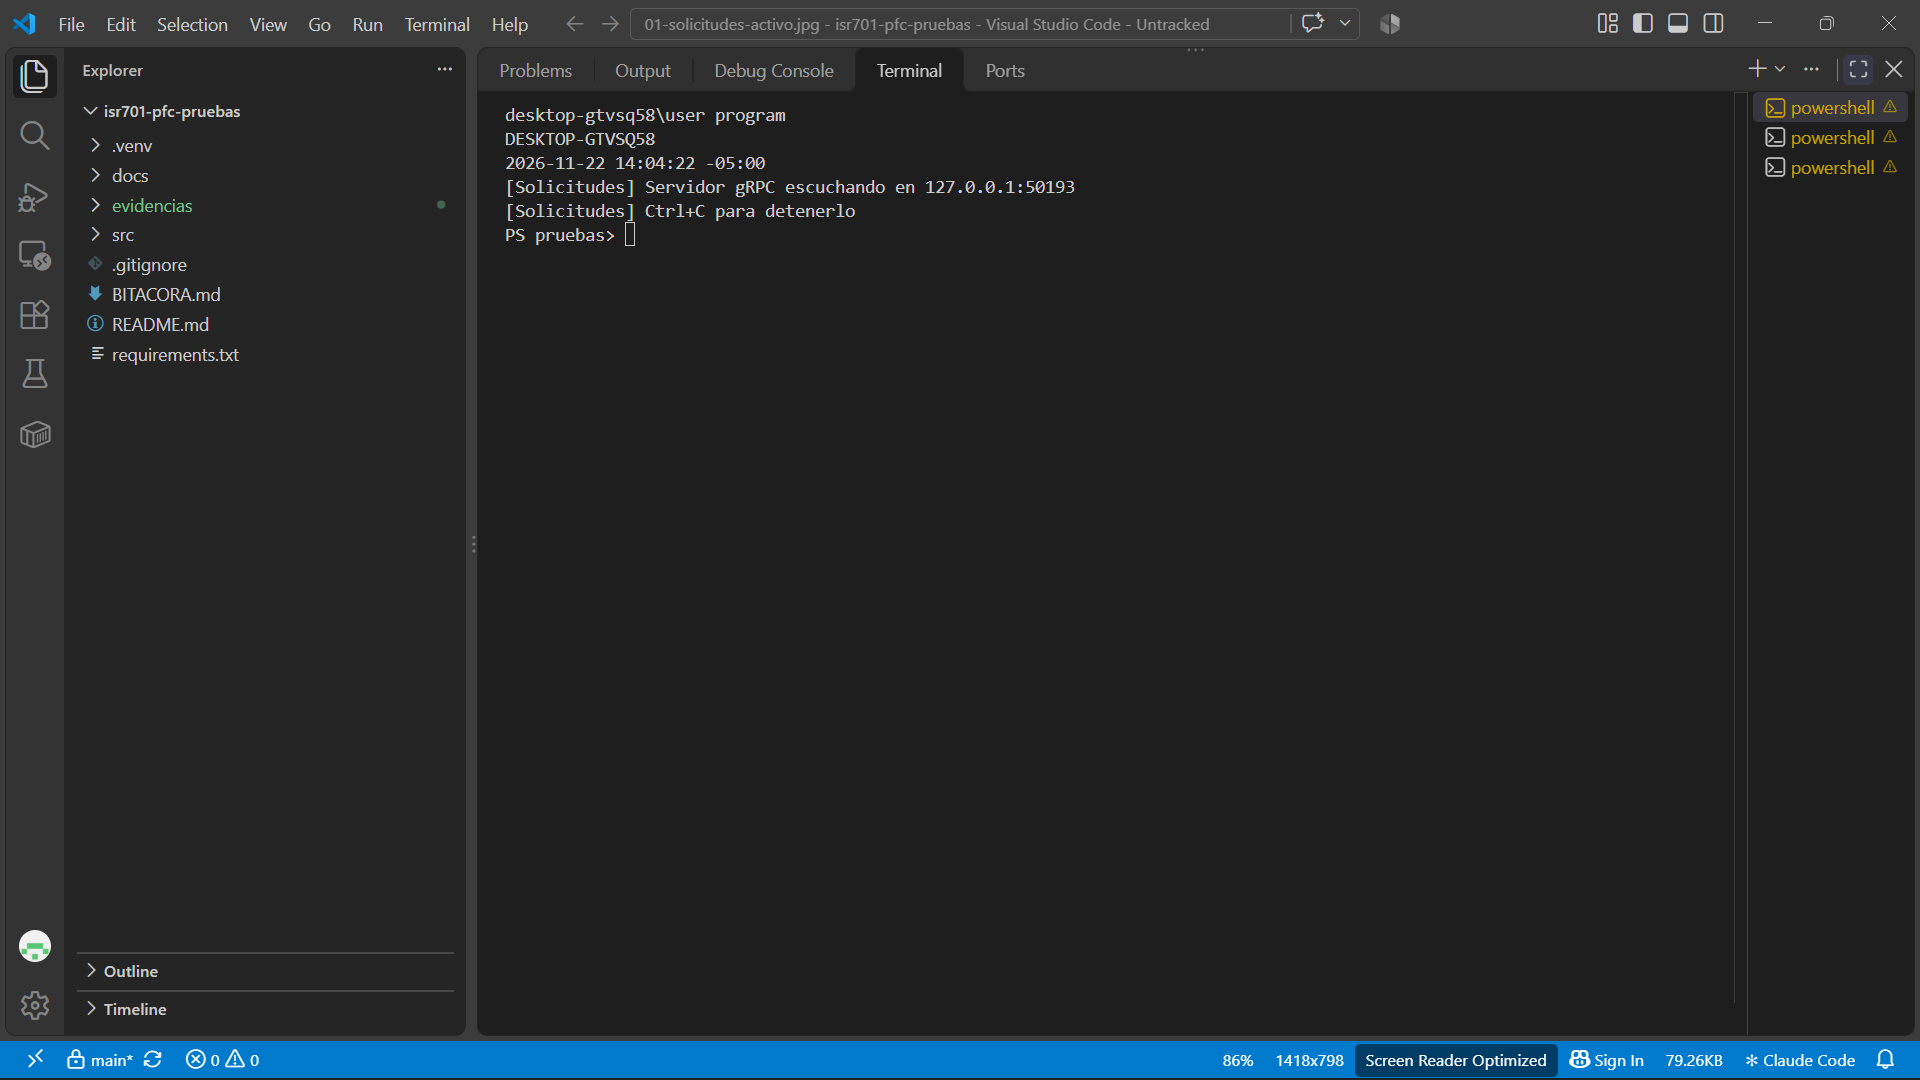
\includegraphics[width=\textwidth]{../evidencias/capturas/01-solicitudes-activo.png}
  \caption{Solicitudes escuchando en la máquina de Jilmar.}
  \label{fig:captura-solicitudes}
\end{figure}

\begin{figure}[htbp]
  \centering
  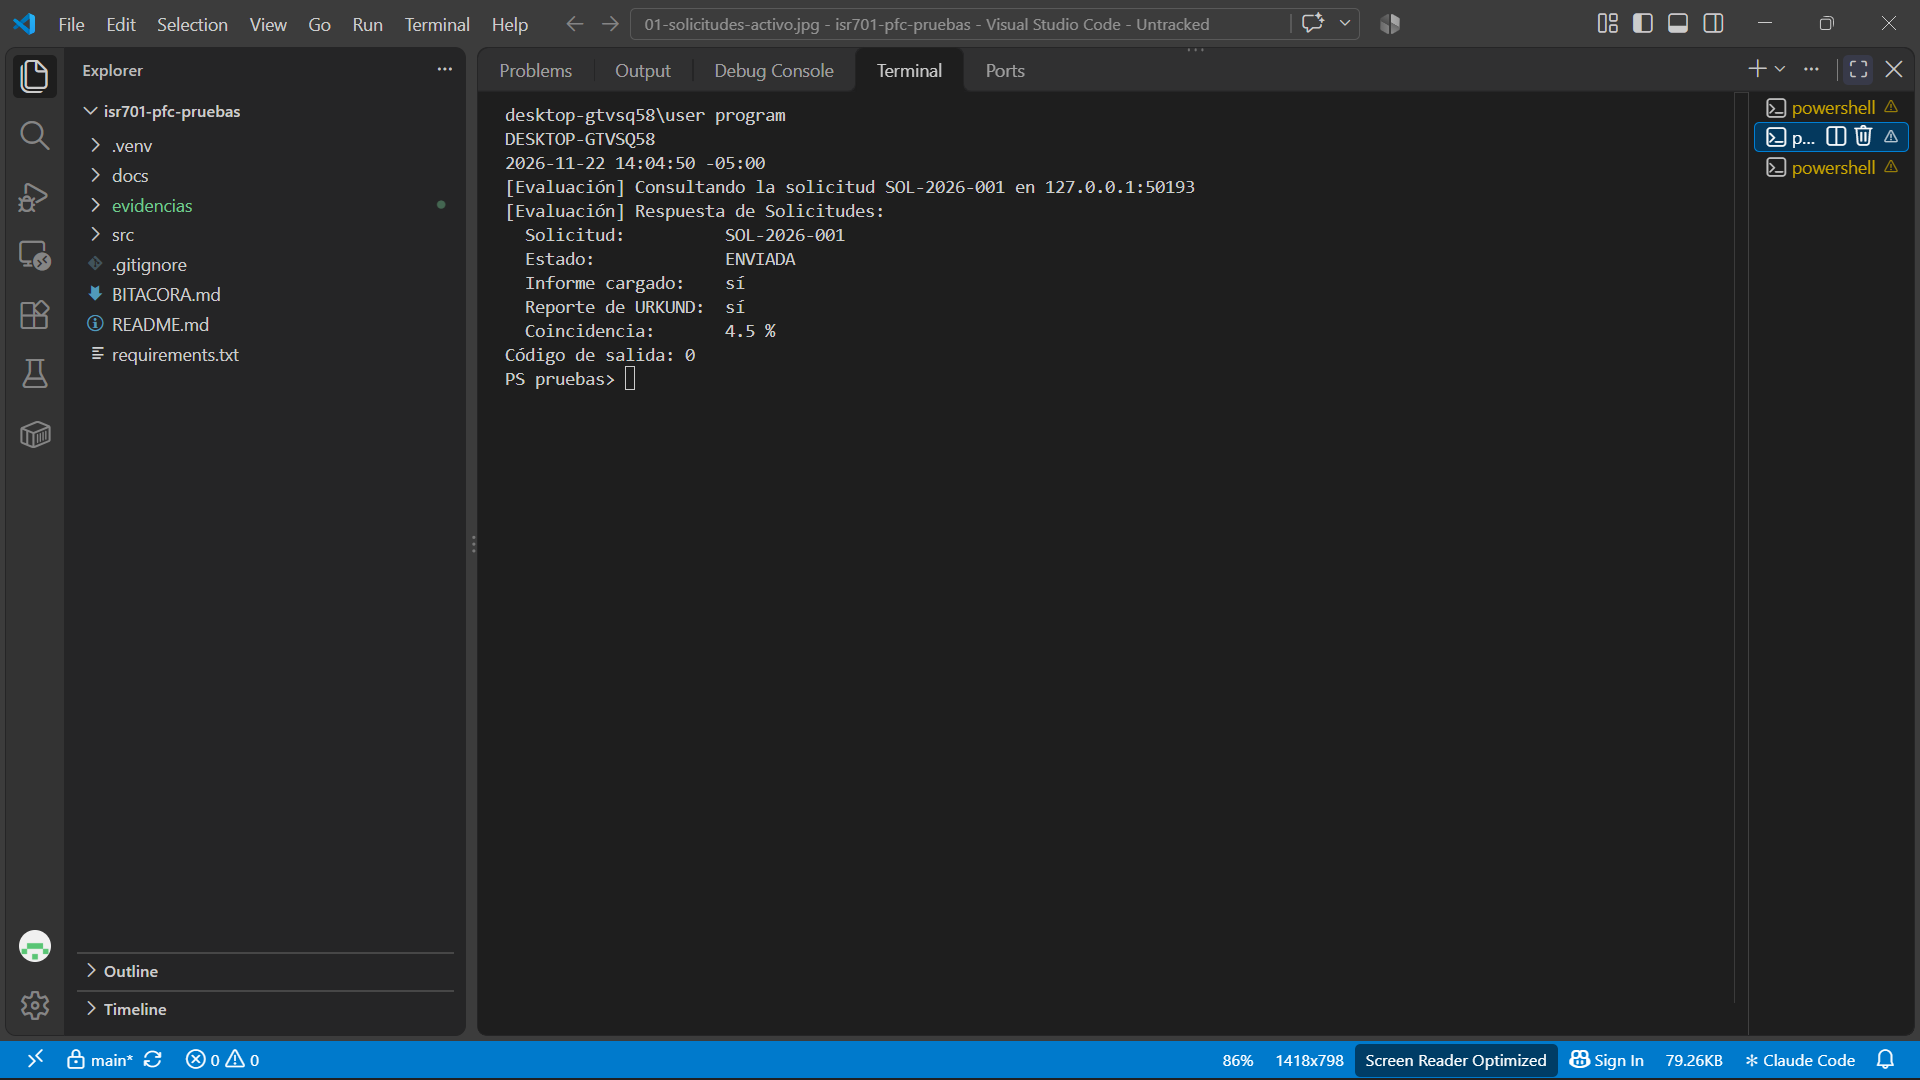
\includegraphics[width=\textwidth]{../evidencias/capturas/02-evaluacion-respuesta.png}
  \caption{Evaluación muestra la respuesta de Solicitudes y termina con código 0.}
  \label{fig:captura-evaluacion}
\end{figure}

\begin{figure}[htbp]
  \centering
  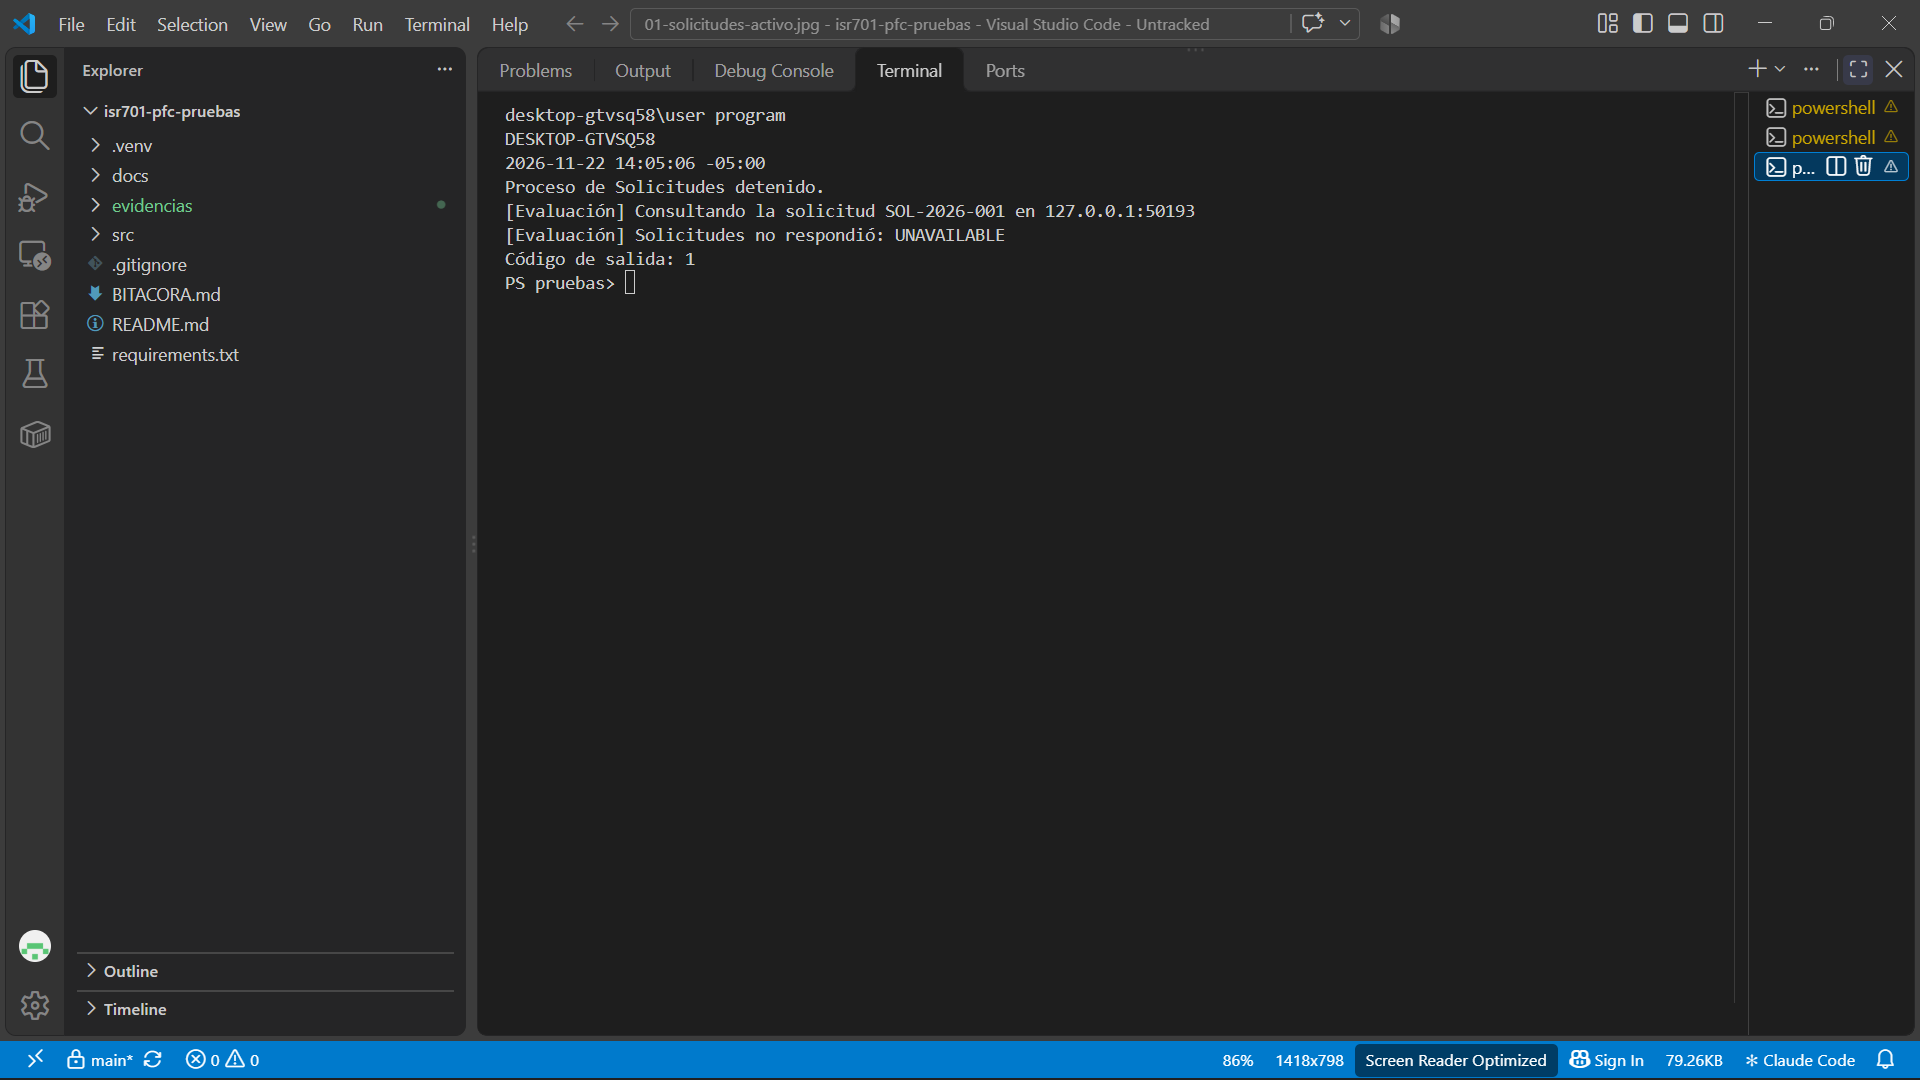
\includegraphics[width=\textwidth]{../evidencias/capturas/03-solicitudes-apagado.png}
  \caption{Con Solicitudes detenido, Evaluación muestra UNAVAILABLE y termina con código 1.}
  \label{fig:captura-apagado}
\end{figure}

\section{Aportes de los integrantes}
\label{sec:aportes}

\begin{xltabular}{\textwidth}{@{} >{\raggedright\arraybackslash}p{2.6cm} >{\raggedright\arraybackslash}p{2.0cm} >{\raggedright\arraybackslash}p{5.5cm} >{\raggedright\arraybackslash}p{3.9cm} @{}}
  \caption{Aporte individual de cada integrante al repositorio.}
  \label{tab:aportes} \\
  \toprule
  \textbf{Integrante} & \textbf{Rol} & \textbf{Qué hizo} & \textbf{Evidencia} \\
  \midrule
  \endfirsthead
  \toprule
  \textbf{Integrante} & \textbf{Rol} & \textbf{Qué hizo} & \textbf{Evidencia} \\
  \midrule
  \endhead
  \bottomrule
  \endfoot

  Dariem Alberto Benites Pérez & Arquitecto &
  Diseñé la arquitectura a partir del bosquejo hecho en grupo y de la
  entrevista: los diagramas C4 de contexto y de contenedores, el ADR-001,
  la justificación frente al monolito, el modelo de comunicación y el
  análisis CAP y PACELC. Apliqué las aclaraciones de la revisión de
  coherencia del issue \#20. &
  Issues \href{https://github.com/reyshadow0/isr701-pfc/issues/1}{\#1}, \href{https://github.com/reyshadow0/isr701-pfc/issues/2}{\#2}, \href{https://github.com/reyshadow0/isr701-pfc/issues/3}{\#3}, \href{https://github.com/reyshadow0/isr701-pfc/issues/4}{\#4}, \href{https://github.com/reyshadow0/isr701-pfc/issues/5}{\#5}, \href{https://github.com/reyshadow0/isr701-pfc/issues/6}{\#6}, \href{https://github.com/reyshadow0/isr701-pfc/issues/7}{\#7}.
  Commits \href{https://github.com/reyshadow0/isr701-pfc/commit/1cbaf8b}{\texttt{1cbaf8b}}, \href{https://github.com/reyshadow0/isr701-pfc/commit/882ec3d}{\texttt{882ec3d}}, \href{https://github.com/reyshadow0/isr701-pfc/commit/8aaae57}{\texttt{8aaae57}}, \href{https://github.com/reyshadow0/isr701-pfc/commit/0251f4b}{\texttt{0251f4b}}, \href{https://github.com/reyshadow0/isr701-pfc/commit/b90472f}{\texttt{b90472f}}, \href{https://github.com/reyshadow0/isr701-pfc/commit/43df3f0}{\texttt{43df3f0}}, \href{https://github.com/reyshadow0/isr701-pfc/commit/7792865}{\texttt{7792865}}, \href{https://github.com/reyshadow0/isr701-pfc/commit/42b682d}{\texttt{42b682d}}.
  PR \href{https://github.com/reyshadow0/isr701-pfc/pull/36}{\#36}, \href{https://github.com/reyshadow0/isr701-pfc/pull/37}{\#37}, \href{https://github.com/reyshadow0/isr701-pfc/pull/38}{\#38}, \href{https://github.com/reyshadow0/isr701-pfc/pull/44}{\#44}, \href{https://github.com/reyshadow0/isr701-pfc/pull/45}{\#45}. \\
  \addlinespace

  % Filas de Mario, Jilmar y Steven: cada uno agrega la suya con su propio texto.

\end{xltabular}

\section{Declaración de uso de inteligencia artificial}
\label{sec:declaracion-ia}

\begin{xltabular}{\textwidth}{@{} >{\raggedright\arraybackslash}p{2.2cm} >{\raggedright\arraybackslash}p{2.4cm} >{\raggedright\arraybackslash}p{1.7cm} >{\raggedright\arraybackslash}p{3.6cm} >{\raggedright\arraybackslash}p{3.8cm} @{}}
  \caption{Herramientas de inteligencia artificial usadas como apoyo.}
  \label{tab:declaracion-ia} \\
  \toprule
  \textbf{Integrante} & \textbf{Herramienta} & \textbf{Versión} & \textbf{Para qué se usó} & \textbf{Cómo se verificó lo obtenido} \\
  \midrule
  \endfirsthead
  \toprule
  \textbf{Integrante} & \textbf{Herramienta} & \textbf{Versión} & \textbf{Para qué se usó} & \textbf{Cómo se verificó lo obtenido} \\
  \midrule
  \endhead
  \bottomrule
  \endfoot

  Steven Pozo & OpenAI Codex & GPT-5 &
  Organización y redacción de borradores del resumen de la entrevista,
  contexto, historias de usuario y trabajos relacionados; búsqueda y
  revisión de referencias; apoyo inicial en la bitácora. &
  Contrastó los borradores con los datos entregados por el equipo, mantuvo
  como pendientes los datos no confirmados, verificó los DOI contra las
  páginas de las revistas y revisará el contenido con el equipo y la
  entrevistada antes de usarlo como evidencia. \\
  \addlinespace

  Dariem Benites & Claude Code (Anthropic) & Claude Opus 5.5 &
  Usé Claude para que me ayude a corregir los borradores del ADR-001 y
  de las secciones 06, 07, 08, 09 y 10a con la entrevista, los RNF y los
  riesgos; resumir el artículo de Blinowski et al.; pasar tablas a
  xltabular y compilar; revisar la coherencia con los RNF y los riesgos, y
  aplicar pequeñas correcciones a las aclaraciones del \#20. &
  Comparé los diagramas con mi bosquejo, la entrevista y las correcciones
  de Mario; revisé cada cifra contra la entrevista y la sección 05;
  comprobé las referencias con su DOI; compilé sin errores y revisé tablas
  y figuras en el PDF; y leí cada sección hasta poder explicarla. \\
  \addlinespace

  Jilmar Cedeño & OpenAI Codex & GPT-6.2 ligero &
  Usé Codex para preparar y ajustar borradores de objetivos, requisitos no
  funcionales y riesgos, y para comparar las secciones en la revisión del
  issue \#20. &
  Contrasté los datos de los requisitos no funcionales con la entrevista y
  comprobé los hallazgos en las secciones 08 y 09, el riesgo R02 y el
  ADR-001. \\
  \addlinespace

  Mario Castro & Claude (Anthropic) & Claude Opus 5.5 &
  Usé Claude como apoyo. La elección de gRPC y el alcance del esqueleto ya
  los habíamos decidido en el equipo (issues \#10 y \#11). Escribí
  una primera versión del código, basada en la de PE-U1, y borradores del
  ADR-002, de las secciones 10b, 12 y 13 y del README, y Claude corrigió el formato de las tablas de aportes y de declaración de IA (xltabular), resolvió los conflictos al fusionar las ramas del equipo y compiló el documento varias veces. En esas compilaciones encontró varios errores: la versión de Python estaba mal puesta, había un desborde de medio punto y un proceso se había quedado colgado en el puerto 50051. &
  Seguí solo el README en un clon limpio, en Windows~11, el 21 de noviembre
  de 2026, y comprobé los cuatro pasos, incluido el de Solicitudes
  apagado. Contrasté el ADR-002 con el código de sockets y gRPC de PE-U1 y
  con las secciones 08 y 09, y dejé pendientes las cifras de latencia hasta
  tener la corrida oficial. Compilé el documento y revisé las secciones en
  el PDF. \\
  \addlinespace

\end{xltabular}


\printbibliography[heading=bibintoc,title={Referencias}]

\end{document}
